\begin{frame}
\frametitle{Régulation}
\framesubtitle{Introduction}
Quelques questions à se poser :
\begin{itemize}
	\item Où veut-on aller ?
	\item Comment commander les moteurs ?
	\item Vers où le robot se dirige-t-il ? Où est-il par rapport à l'objectif ?
	\item Il y a-t-il un obstacle devant le robot ?
	\item Pourquoi a-t-on besoin d'une régulation ?
\end{itemize}
\end{frame}

\begin{frame}
\frametitle{Régulation}
\framesubtitle{Consigne et commande des moteurs}
La consigne est reçue via l'I\up{2}C, on a disposition :
\begin{itemize}
	\item La fonction (4bits), choix de la commande;
	\item Les données (12bits), distance à parcourir.
\end{itemize}
\begin{table}[!ht]
	\centering
	\begin{tabular}{|l|cc|cc|}
		\hline
		& DIR1 & DIR2 & PWM1 & PWM2 \\
		\hline
		Forward & 1 & 1 & \multicolumn {2}{c|}{Variable} \\
		\hline
		Backward & 0 & 0 & \multicolumn {2}{c|}{Variable} \\
		\hline
		Turn Left & 1 & 0 & \multicolumn {2}{c|}{Variable} \\
		\hline
		Turn Right & 0 & 1 & \multicolumn {2}{c|}{Variable} \\
		\hline
		Stop & \multicolumn {2}{c|}{X} & 0 & 0 \\
		\hline
	\end{tabular}
	\caption{Commandes des moteurs}
\end{table}
\end{frame}

\begin{frame}
\frametitle{Régulation}
\framesubtitle{Roues codeuses et capteurs ultrasons}
Capteurs ultrasons : uniquement en cas d'arrêt d'urgence.\\
Roues codeuses :
\begin{itemize}
	\item 1024 tics par tour ;
	\item 20 cm par tour.
\end{itemize}
\begin{figure}[!ht]
	\centering
	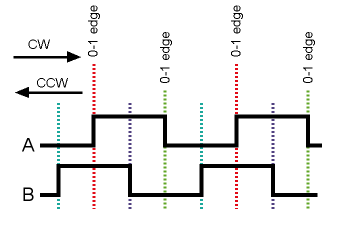
\includegraphics[scale=0.5]{roues_codeuses.png}
	\caption{Signal des roues codeuses}
\end{figure}
\end{frame}

\begin{frame}
\frametitle{Régulation}
\framesubtitle{Schéma bloc}
\begin{figure}[!ht]
	\centering
	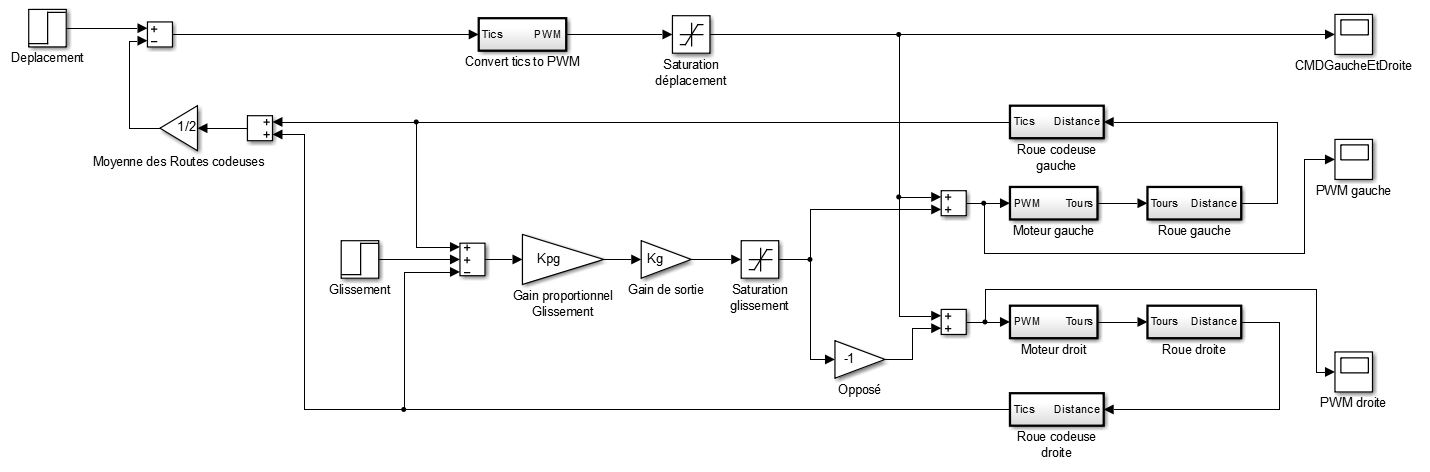
\includegraphics[scale=0.28]{simulink.jpg}
	\caption{Schéma bloc de la régulation des moteurs}
	\label{img:simulink}
\end{figure}
\end{frame}

\begin{frame}
\frametitle{Régulation}
\framesubtitle{Coefficients Kp et Kig}
\begin{description}
	\item[Kp] Coefficient proportionnel du déplacement; 
			\hfill \\ Ralentir la commande en se rapprochant. 
	\item[Kig] Coefficient intégrateur du glissement;
			\hfill \\ Éviter les variations entre la rotation des moteurs et la rotation des roues.
\end{description}
\end{frame}